\documentclass[11pt]{beamer}
\usepackage[utf8]{inputenc}
\usepackage[T1]{fontenc}
\usepackage{lmodern}
\usepackage[french]{babel}
\usepackage{minted}
\usepackage{amsthm}
\usepackage{multicol}
\usepackage{verbatim}
\usepackage{tikz}
\usetikzlibrary{arrows}
\usetikzlibrary{tikzmark}

\usetheme{default}

\newminted[myocaml]{ocaml}{texcl=true, escapeinside=??}
\newenvironment{ocaml}
{\small\VerbatimEnvironment
	\begin{myocaml}}
	{\end{myocaml}}
\newminted[mytinyocaml]{ocaml}{texcl=true, fontsize=\scriptsize}
\newenvironment{tinyocaml}
{\small\VerbatimEnvironment
	\begin{mytinyocaml}}
	{\end{mytinyocaml}}

\setbeamertemplate{footline}[frame number]

\begin{document}
	\author{Alexandre Moine \& Yann Régis-Gianas}
	\title{Détection de définitions OCaml similaires}
	\subtitle{(ou comment ne plus voir double à dos de chameau)}
	%\logo{}
	\institute{Université de Paris -- IRIF -- INRIA $\pi.r^2$ -- Fondation OCaml}
	\date{Vendredi 31 janvier 2020}
	%\subject{}
	%\setbeamercovered{transparent}
	%\setbeamertemplate{navigation symbols}{}
	\begin{frame}[plain]
		\maketitle
	\end{frame}

\section{Introduction}

\section{Overview}
\subsection{LearnOCaml}
\begin{frame}
	\frametitle{Le supplice des professeurs}
\begin{center}
\Large
Comment analyser les 150 copies hebdomadaires \\ du cours de programmation fonctionnelle ?
\end{center}
\pause
\bigskip
\begin{itemize}
\item Utiliser LearnOCaml\only<2->{\footnote{https://github.com/ocaml-sf/learn-ocaml}}.
\pause
\item Mais 75\% des élèves ont tout juste.
\item Comment appréhender \emph{le raisonnement} de l'élève pour mieux comprendre leurs
  difficultés et leur proposer des exercices adaptés?
\end{itemize}
\end{frame}

\begin{frame}
	\frametitle{Comment ferait un professeur un peu mécanique ?}
	\begin{enumerate}
		\item Regarder uniquement la "forme" des fonctions.
		\item Identifier celles ayant exactement la même forme.
		\item Essayer de trouver celles ayant des formes ressemblantes.
	\end{enumerate}
\end{frame}

\begin{frame}[fragile]
	\frametitle{Un exemple}
	\framesubtitle{List.rev par des étudiants}

\begin{multicols}{2}
\begin{tinyocaml}
(* Code 1 *)
let rec rev l = match l with
  [] -> []
  |t::q -> rev q@[t]

(* Code 2 *)
let rec rev l = match l with
  | [] -> []
  | a::t -> (rev t)@[a]

(* Code 3 *)
let rec rev l = match l with
  [] | [_] -> l
  | t::q -> rev q@[t];;
\end{tinyocaml}
\begin{figure}
	\begin{center}
		\begin{tikzpicture}[sloped, scale=0.4]
		\node (a)  at (-6,0)   {1};
		\node (b)  at (-5,0)   {2};
		\node (ab) at (-5.5,1) {};
		\node (c) at (-3,0) {3};
		\node (abc) at (-4, 2) {};
		\node (d) at (-2,0) {4};
		\node (e) at (-1,0) {5};
		\node (de) at (-1.5,2) {};
		\node (f) at (0,0) {6};
		
		\draw  (a) |- (ab.center);
		\draw  (b) |- (ab.center);
		\draw  (ab) |- (abc.center);
		\draw  (c)  |- (abc.center);
		\draw  (d)  |- (de.center);
		\draw  (e)  |- (de.center);
		
		\draw[->,-triangle 60] (-7,0) -- node[above]{dissimilarité} (-7,3);
		\end{tikzpicture}
	\end{center}
\end{figure}
\columnbreak
\begin{tinyocaml}
(* Code 4 *)
let rev l=
  let rec rev_aux acc l= match l with
    |[]->acc
    |t::q->rev_aux (t::acc) q
  in rev_aux [] l

(* Code 5 *)
let rev l = match l with
  [] -> []
  |a::q ->
    let rec rev2 x y = match y with
    [] -> x
    |b::z -> rev2 (b::x) z in rev2 [] l

(* Code 6 *)
let rev l = List.fold_left
    (fun acc x -> x :: acc) [] l
\end{tinyocaml}
\end{multicols}

\end{frame}

\begin{frame}[fragile]
	\frametitle{Asak à la rescousse}
	\begin{itemize}
		\item Asak, une bibliothèque qui suit cette méthodologie:
		\begin{center}
                  \url{https://github.com/nobrakal/asak}
                \end{center}
		\item Disponible sur OPAM et intégrée dans LearnOCaml.
		\item Elle produit des \emph{dendrogrammes} à partir d'un corpus.
	\end{itemize}
\bigskip
\pause
	Asak vient aussi avec:
	\begin{itemize}
		\item Des outils pour compiler tout le dépôt OPAM et y analyser la redondance.
		\item Un exécutable \verb|anzad| qui permet d'analyser la redondance d'un projet construit avec \verb|dune|.
	\end{itemize}
\end{frame}

\subsubsection{La forme}

\begin{frame}
\frametitle{La forme des fonctions}
Comment capturer la "forme" des fonctions ?
\begin{itemize}
\item Le texte ? \only<2->{\alert{On ne veut prendre en compte que le code.}}
\item Une analyse lexicale ? \only<3->{\alert{$\alpha$-conversion ? $\beta$-réduction ?}}
\item Une analyse syntaxique ? \only<5->{\alert{Pas trop mal...}}
\item Les graphes de dépendances ? \only<4->{\alert{Trop compliqué !}}
\end{itemize}
\end{frame}

\begin{frame}
\frametitle{Les arbres de syntaxe abstraits}
\begin{itemize}
\item L'arbre de syntaxe abstrait d'OCaml est trop:
	\begin{itemize}
		\item Riche: différence match/function.
		\item Difficile à manipuler.
	\end{itemize}
\pause
\item Une solution: \alert{utiliser Lambda}.
	\begin{itemize}
	\item Un langage intermédiaire de la compilation d'OCaml.
	\item Un $\lambda$-calcul enrichi.
\end{itemize}
\pause
\item Avantages:
\begin{itemize}
	\item Plus concis que l'AST d'OCaml.
	\item Issue d'une première passe de compilation.
\end{itemize}
\end{itemize}
\end{frame}

\subsubsection{Les définitions identiques}
\begin{frame}
\frametitle{Un problème d'arbre}
\begin{itemize}
\item "Mêmes" arbres Lambda $\sim$ fonctions identiques
\item Comment capturer la forme des arbres ?
\pause
\item[$\Rightarrow$] via leurs \emph{empreintes}.
\end{itemize}
\end{frame}

\subsubsection{Les définitions similaires}
\begin{frame}
	\frametitle{À propos de partitions}
On veut partitionner les copies selon une notion de \emph{dissimilarité}:
\begin{itemize}
\item Grouper les définitions "proches" jusqu'à obtenir des groupes très distincts.
\item Il s'agit de faire un partitionnement hiérarchique \emph{ascendant}.
\end{itemize}
\end{frame}

\begin{frame}
\frametitle{Démonstration}
\end{frame}

\subsection{Détéction de redondance}
\begin{frame}
\frametitle{Une chose en entrainant une autre...}

\begin{itemize}
\item Pouvoir regrouper les copies étudiantes par similarité est une bonne chose.
\item L'approche choisie permet en fait d'étudier la similarité de \emph{n'importe quel} corpus.
\item Et pourquoi pas l'ensemble des paquets OPAM ?
\end{itemize}
\end{frame}

\begin{frame}
	\frametitle{Analyse des paquets OPAM}
	\begin{itemize}
		\item 1250 paquets \textcolor{gray}{/ 2569}
		\item 374 959 définitions let
		\item 172 412 classes différentes
		\item 48 841 classes non triviales
	\end{itemize}
\pause
Après quelques raffinements (suppression du code généré, des copié/collé (MyOcamlBuild...))
\begin{itemize}
	\item 102 805 définitions let
	\item 2 973 classes différentes
\end{itemize}
\pause
Il y a encore du tri à faire.
\end{frame}

\begin{frame}[fragile]
	\frametitle{Option.map ?}
	\begin{itemize}
		\item 140 occurrences
		\item 32 noms différents !
	\end{itemize}
	\pause
	\begin{footnotesize}
		\begin{multicols}{3}
			\begin{itemize}
				\item apply\_opt
				\item applyOption
				\item app\_opt
				\item copy\_option
				\item flatten\_option
				\item fmap
				\item fopt
				\item lift\_opt map 
				\item map\_evar\_body
				\item map\_of\_option
				\item map\_opt
				\item map\_option
				\item map\_some
				\item may
				\item may\_apply
				\item maybe
				\item may\_map
				\item oapply
				\item omap
				\item opt
				\item opt\_apply
				\item option
				\item option\_map
				\item optionMap
				\item option\_of\_comp
				\item \_opt\_map
				\item opt\_map
				\item opt\_wrap
				\item sure
				\item u\_option
				\item vof\_option
			\end{itemize}
		\end{multicols}
	\end{footnotesize}

\end{frame}

\begin{frame}[fragile]
\frametitle{RosettaCode}
\begin{Verbatim}[fontsize=\footnotesize]
alba.0.4.0:container.ml:
  Container:Container.levenshtein_distance
cmdliner.1.0.4:cmdliner_suggest.ml:
  Cmdliner_suggest:Cmdliner_suggest.levenshtein_distance
dune.1.11.3:src.stdune.user_message.ml:
  Stdune__User_message:Stdune__User_message.levenshtein_distance
dune.1.11.3:vendor.cmdliner.src.cmdliner_suggest.ml:
  Cmdliner_suggest:Cmdliner_suggest.levenshtein_distance
omod.0.0.2:src.omod.ml:
  Omod:Omod.String.edit_distance
opam-depext.1.1.3:cmdliner.src.cmdliner.ml:
  Cmdliner:Cmdliner.levenshtein_distance
reason.3.5.0:src.reason-parser.vendor.cmdliner.vendored_cmdliner.ml:
  Vendored_cmdliner:Vendored_cmdliner.levenshtein_distance
\end{Verbatim}
Des copiés-collés de \url{http://rosettacode.org/wiki/Levenshtein_distance#OCaml}
\end{frame}

\section{Détails techniques}

\begin{frame}
\frametitle{Principe de fonctionnement de l'approche}
	\begin{enumerate}
	\item Compiler le corpus vers Lambda.
	\item Normaliser les arbres obtenus.
	\item Prendre les empreintes des arbres.
	\item Grouper par empreintes identiques.
	\item Faire un partitionnement par ressemblance.
\end{enumerate}
\end{frame}

\subsection{Lambda}
\begin{frame}[fragile]
\frametitle{Lambda}
Par rapport à OCaml:
\begin{itemize}
	\item Non typé.
	\item Absence du langage des modules.
	\item Absence de filtrage par motif.
\end{itemize}
\pause
Cela nous permet d'identifier les types isomorphes !
\begin{ocaml}
let map_evar_body f = function
  Evar_empty     -> Evar_empty 
| Evar_defined d -> Evar_defined (f d)
\end{ocaml}

\begin{multicols}{2}
\begin{ocaml}
let map_opt f = function
  None -> None
| Some x -> Some (f x)
\end{ocaml}
$ $\\
\begin{verbatim}
function f/88 param/90 
  (if 1/93 
    (makeblock 0 
      (apply 2/92 
        (field 0 1/91)))
    0a)
\end{verbatim}

\end{multicols}

\end{frame}

\begin{frame}[fragile]
\frametitle{Lambda \alert{normalisé}}
\begin{itemize}
	\item $\alpha$-renommage des variables locales (via indice de de Bruijn).
\begin{center}
\begin{tikzpicture}[sibling distance=5em, every node/.style = {shape=rectangle,
	draw, align=center}]]
\node (A) at (-5,0) {let x}
child { node {f ()} }
child { node {let y}
  child {node {g x}}
  child {node {x + y}}
};

\node (B) at (0,0) {let \_1}
child { node {f ()} }
child { node {let \_2}
	child {node {g \_1}}
	child {node {\_2 + \_1}}
};

\draw[thick,red,->,>=latex] (A) -- (B);
\end{tikzpicture}
\end{center}
	\item Réduction des définitions locales inoffensives:
	
\begin{multicols}{2}
\begin{ocaml}
let f x =             ?\tikzmark{A}?
  let u = 1 in u + x
\end{ocaml}
\columnbreak
\begin{ocaml}
?\tikzmark{B}?  let f x =
    1 + x
\end{ocaml}
\end{multicols}
\end{itemize}

\begin{tikzpicture}[remember picture]
\draw[auto=right,overlay,thick,red,->,>=latex] (pic cs:A) -- (pic cs:B);
\end{tikzpicture}
\end{frame}

\subsection{Prises d'empreintes}
\begin{frame}
	\frametitle{Prise d'empreinte}
	Comment comparer deux arbres ?
	
	\pause
	
	On calcule \alert{récursivement} des empreintes.
	\pause
	
	\begin{itemize}
		\item On définit une empreinte pour les feuilles.
		\item On calcule l'empreinte d'un nœud à partir des empreintes de ses sous-arbres.
	\end{itemize}
	
	\pause
	À empreinte de racine égale, arbre égal.
	
\end{frame}

\begin{frame}
	\frametitle{Objectif similarité}
	Comment voir si deux arbres partagent des sous-arbres ?
	
	\begin{itemize}
		\item On conserve les empreintes des sous-arbres.
		\item Avec un poids: le nombre de nœuds.
	\end{itemize}

On a donc:
$$E : Lambda \to Bag(\mathbb{N} \times \mathbb{N})$$
Attention, il s'agit d'un multi-ensemble !
\end{frame}

\begin{frame}
\tiny\begin{multicols}{2}
\[\begin{array}{rcl}
01 &=& 6cdbdd45d9fda8de7da9dc4d9add5d43d4ad80d44df9d9cd \\
02 &=& 58de8dc8d46d83d87d4bd23d24d93d82d69de2d32d64dc6d \\
03 &=& dddc1d3dd8adf7d7d41d4dd8bd9d2ed30d6edf4d9fd2d \\
04 &=& 64dc6d47d3adf8d15dc5d28d5d2bd12d6d7dda2d74dc6d \\
05 &=& 89db7df1d30df9d8adfddbfd6bdf8dc5decd66d13dbed5ad \\
06 &=& acdadd7ddebd3dd8fd21da4d71d4fdd2db4dbcde0d10d68d \\
07 &=& 72dfd3cdfad34d33de1d4fd46d4dd9cdcbd9cd77d12d32d \\
08 &=& dfddd6edefd9ddbddffde0dc3d11d58d8cdcdb5d73dafd \\
09 &=& 78da6d29de0d96dabd9fd2d71d9fdcdd9db7d3ad74dfcd \\
10 &=& 5ed72d97d35db8d71d1cdb6d79de7dbcd3ad19dfdd8dd56d \\
11 &=& 8bda1d14d86d29df2da7d7dda0d4dd5addad5fd2d1fdddd \\
12 &=& d4d1dd8cdd9d8fd0db2d4de9d80d9d98decdf8d42d7ed \\
13 &=& cbdccdbfdfcddbd7dd7ed77d39dc4d27d8dda1d25d4ed86d \\
14 &=& dad42decd1cd57df0d66df4ddadc1d72d29d42db3dfad7ed \\
15 &=& afd20d78d4fdbdd60d83d7fda3d30d5adcbdc3d3dd82de0d \\
16 &=& 72d64d45d84d18d55dabde6d2bd29dfad1fd55dc7de4d15d \\
17 &=& e6d95d5bdaadc8dc2d9fd33d7dd4dd1edacd10deed67d76d \\
18 &=& 36d80d66d3fd81defd16d12d16ddedb7dbbd94d2ed7dd11d \\
19 &=& bad43dccdcdd18d52d3bd82d2ada8d0d8ed90da8dc2dd0d \\

\end{array}\\
\begin{array}{rcl}
20 &=& cfd38df3df7d42dc0ddbdd5d53de6d9bd39d6adfcd6ad20d \\
21 &=& b2dfddb8d99dccd8adc5d6edacde2d26d66dcdd7cdaed39d \\
22 &=& 47db7dbed82dd0d84d17d51d8fdd9db1de1d45d39d6ad38d \\
23 &=& ad14d0d7cd4ed7de9dd3d4cde6d20de6d57df1dcade0d \\
24 &=& c5d34dccd9fdc4d9d96d6ddcfd44d82d5cd19db5dd6dd6d \\
25 &=& 1fd53d57dceda3df6daed5fdb8de6d7fdc4d61dafde8d96d \\
26 &=& 18dedb6dcddc4d69d33d9bd5bdcad46df0d56d8fd1dc5d \\
27 &=& f1d4fdad1ed86db0d7dd2fd41df1df4d1fd25d36d46d54d \\
28 &=& 42d45d6dd2fd86d91d1dd78dd6dfdd2ed4fd4ad1d20d24d \\
29 &=& 6bdcad8dd97d19dc8d86d87d95d1ddf1d49dedd17d91d5dd \\
30 &=& ebd8cd7ed71de9d71d65dc2d33d65d57d11de5df3d7ad73d \\
31 &=& e0dbbdefd1ddfed38d27d22d0df4dd6dddacde3dcbd77d \\
32 &=& 3adebdc5dc4d4ad5addadf6d9ad8fde4d38decd50d90da5d \\
33 &=& 39d7d29d5dcdd80dddddedd5de3d5dda3d2ad57d4ed96d \\
34 &=& a8d7bdccda2d93d67d2ddaed34d38df1de2dbad95d3ad41d \\
35 &=& 6adf1d16daedc3d80db8dc8d3da2dfbde9dd7d84d72d83d \\
36 &=& f1dead89d1cd13dd6db9d8fde6d73d19d44d2bd11d90dcbd \\
37 &=& 81d72d4dd8cdbcdd5db6d43d86d2fd75dddd2dd85d67dbcd \\
38 &=& 5edf5d2ed7cd37d4cdded6bd3edd8d94dd6d4cdbad79d95d \\
39 &=& 20d57df0dbfd84df5d8bdecd92d6dd5ed22d4fd6d58debd \\
\end{array}\\
\]\end{multicols}
\[\begin{array}{rcl}
E(D_1) &=& \{ \begin{bmatrix} 13 \\ 20 \end{bmatrix} \begin{bmatrix} 01 \\ 19 \end{bmatrix}\,\begin{bmatrix} 02 \\ 1 \end{bmatrix}\,\begin{bmatrix} 03 \\ 16 \end{bmatrix}\,\begin{bmatrix} 04 \\ 5 \end{bmatrix}\,\begin{bmatrix} 05 \\ 3 \end{bmatrix}\,\begin{bmatrix} 06 \\ 2 \end{bmatrix}\,\begin{bmatrix} 02 \\ 1 \end{bmatrix}\,\begin{bmatrix} 07 \\ 6 \end{bmatrix}\,\begin{bmatrix} 08 \\ 5 \end{bmatrix}\,\begin{bmatrix} 09 \\ 1 \end{bmatrix}\,\begin{bmatrix} 05 \\ 3 \end{bmatrix}\,\begin{bmatrix} 06 \\ 2 \end{bmatrix}\,\begin{bmatrix} 02 \\ 1 \end{bmatrix}\,\begin{bmatrix} 10 \\ 3 \end{bmatrix}\,\begin{bmatrix} 11 \\ 2 \end{bmatrix}\,\begin{bmatrix} 12 \\ 1 \end{bmatrix}\,\begin{bmatrix} 09 \\ 1 \end{bmatrix} \} \\[1em]
E(D_2) &=& \{ \begin{bmatrix} 13 \\ 20 \end{bmatrix} \begin{bmatrix} 01 \\ 19 \end{bmatrix}\,\begin{bmatrix} 02 \\ 1 \end{bmatrix}\,\begin{bmatrix} 03 \\ 16 \end{bmatrix}\,\begin{bmatrix} 04 \\ 5 \end{bmatrix}\,\begin{bmatrix} 05 \\ 3 \end{bmatrix}\,\begin{bmatrix} 06 \\ 2 \end{bmatrix}\,\begin{bmatrix} 02 \\ 1 \end{bmatrix}\,\begin{bmatrix} 07 \\ 6 \end{bmatrix}\,\begin{bmatrix} 08 \\ 5 \end{bmatrix}\,\begin{bmatrix} 09 \\ 1 \end{bmatrix}\,\begin{bmatrix} 05 \\ 3 \end{bmatrix}\,\begin{bmatrix} 06 \\ 2 \end{bmatrix}\,\begin{bmatrix} 02 \\ 1 \end{bmatrix}\,\begin{bmatrix} 10 \\ 3 \end{bmatrix}\,\begin{bmatrix} 11 \\ 2 \end{bmatrix}\,\begin{bmatrix} 12 \\ 1 \end{bmatrix}\,\begin{bmatrix} 09 \\ 1 \end{bmatrix} \} \\[1em]
E(D_3) &=& \{ \begin{bmatrix} 18 \\ 29 \end{bmatrix} \begin{bmatrix} 14 \\ 28 \end{bmatrix}\,\begin{bmatrix} 15 \\ 26 \end{bmatrix}\,\begin{bmatrix} 02 \\ 1 \end{bmatrix}\,\begin{bmatrix} 16 \\ 22 \end{bmatrix}\,\begin{bmatrix} 05 \\ 3 \end{bmatrix}\,\begin{bmatrix} 06 \\ 2 \end{bmatrix}\,\begin{bmatrix} 02 \\ 1 \end{bmatrix}\,\begin{bmatrix} 03 \\ 16 \end{bmatrix}\,\begin{bmatrix} 04 \\ 5 \end{bmatrix}\,\begin{bmatrix} 05 \\ 3 \end{bmatrix}\,\begin{bmatrix} 06 \\ 2 \end{bmatrix}\,\begin{bmatrix} 02 \\ 1 \end{bmatrix}\,\begin{bmatrix} 07 \\ 6 \end{bmatrix}\,\begin{bmatrix} 08 \\ 5 \end{bmatrix}\,\begin{bmatrix} 09 \\ 1 \end{bmatrix}\,\begin{bmatrix} 05 \\ 3 \end{bmatrix}\,\begin{bmatrix} 06 \\ 2 \end{bmatrix}\,\begin{bmatrix} 02 \\ 1 \end{bmatrix}\,\begin{bmatrix} 10 \\ 3 \end{bmatrix}\,\begin{bmatrix} 11 \\ 2 \end{bmatrix}\,\begin{bmatrix} 12 \\ 1 \end{bmatrix}\,\begin{bmatrix} 17 \\ 2 \end{bmatrix}\,\\ & & \;\;\begin{bmatrix} 12 \\ 1 \end{bmatrix}\,\begin{bmatrix} 17 \\ 2 \end{bmatrix}\,\begin{bmatrix} 12 \\ 1 \end{bmatrix}\,\begin{bmatrix} 02 \\ 1 \end{bmatrix} \} \\[1em]
E(D_4) &=& \{ \begin{bmatrix} 31 \\ 22 \end{bmatrix} \begin{bmatrix} 19 \\ 21 \end{bmatrix}\,\begin{bmatrix} 20 \\ 16 \end{bmatrix}\,\begin{bmatrix} 21 \\ 15 \end{bmatrix}\,\begin{bmatrix} 22 \\ 14 \end{bmatrix}\,\begin{bmatrix} 23 \\ 1 \end{bmatrix}\,\begin{bmatrix} 24 \\ 11 \end{bmatrix}\,\begin{bmatrix} 25 \\ 6 \end{bmatrix}\,\begin{bmatrix} 26 \\ 5 \end{bmatrix}\,\begin{bmatrix} 27 \\ 1 \end{bmatrix}\,\begin{bmatrix} 28 \\ 3 \end{bmatrix}\,\begin{bmatrix} 29 \\ 2 \end{bmatrix}\,\begin{bmatrix} 23 \\ 1 \end{bmatrix}\,\begin{bmatrix} 28 \\ 3 \end{bmatrix}\,\begin{bmatrix} 29 \\ 2 \end{bmatrix}\,\begin{bmatrix} 23 \\ 1 \end{bmatrix}\,\begin{bmatrix} 27 \\ 1 \end{bmatrix}\,\begin{bmatrix} 30 \\ 4 \end{bmatrix}\,\begin{bmatrix} 09 \\ 1 \end{bmatrix}\,\begin{bmatrix} 02 \\ 1 \end{bmatrix} \} \\[1em]
E(D_5) &=& \{ \begin{bmatrix} 33 \\ 25 \end{bmatrix} \begin{bmatrix} 32 \\ 24 \end{bmatrix}\,\begin{bmatrix} 02 \\ 1 \end{bmatrix}\,\begin{bmatrix} 19 \\ 21 \end{bmatrix}\,\begin{bmatrix} 20 \\ 16 \end{bmatrix}\,\begin{bmatrix} 21 \\ 15 \end{bmatrix}\,\begin{bmatrix} 22 \\ 14 \end{bmatrix}\,\begin{bmatrix} 23 \\ 1 \end{bmatrix}\,\begin{bmatrix} 24 \\ 11 \end{bmatrix}\,\begin{bmatrix} 25 \\ 6 \end{bmatrix}\,\begin{bmatrix} 26 \\ 5 \end{bmatrix}\,\begin{bmatrix} 27 \\ 1 \end{bmatrix}\,\begin{bmatrix} 28 \\ 3 \end{bmatrix}\,\begin{bmatrix} 29 \\ 2 \end{bmatrix}\,\begin{bmatrix} 23 \\ 1 \end{bmatrix}\,\begin{bmatrix} 28 \\ 3 \end{bmatrix}\,\begin{bmatrix} 29 \\ 2 \end{bmatrix}\,\begin{bmatrix} 23 \\ 1 \end{bmatrix}\,\begin{bmatrix} 27 \\ 1 \end{bmatrix}\,\begin{bmatrix} 30 \\ 4 \end{bmatrix}\,\begin{bmatrix} 09 \\ 1 \end{bmatrix}\,\begin{bmatrix} 02 \\ 1 \end{bmatrix}\,\begin{bmatrix} 09 \\ 1 \end{bmatrix} \} \\[1em]
E(D_6) &=& \{ \begin{bmatrix} 39 \\ 13 \end{bmatrix} \begin{bmatrix} 34 \\ 12 \end{bmatrix}\,\begin{bmatrix} 35 \\ 5 \end{bmatrix}\,\begin{bmatrix} 36 \\ 4 \end{bmatrix}\,\begin{bmatrix} 37 \\ 3 \end{bmatrix}\,\begin{bmatrix} 23 \\ 1 \end{bmatrix}\,\begin{bmatrix} 38 \\ 1 \end{bmatrix}\,\begin{bmatrix} 09 \\ 1 \end{bmatrix}\,\begin{bmatrix} 02 \\ 1 \end{bmatrix}\,\begin{bmatrix} 10 \\ 3 \end{bmatrix}\,\begin{bmatrix} 11 \\ 2 \end{bmatrix}\,\begin{bmatrix} 12 \\ 1 \end{bmatrix} \} \\[1em]
\end{array}\]

\end{frame}

\begin{frame}
	\frametitle{Plein de paramètres}
	
	\begin{itemize}
		\item Que faire des feuilles:
		\begin{itemize}
			\item Les constantes: Toutes la même empreinte.
			\item Les variables: Empreinte basée sur leur nom.
		\end{itemize}
		\item Combien de sous-empreintes conserver ?
		\item Comment calculer l'empreinte d'une nœud:
		\begin{itemize}
			\item Normalement: L'ordre des sous-empreintes importe.
			\item Sous une hypothèse d'équivalence sémantique: l'ordre n'importe pas !
		\end{itemize}
	\end{itemize}
\end{frame}

\subsection{Partitionnement}

\begin{frame}
	\frametitle{Une semi-métrique}
	\begin{definition}[Dissimilarité]
		$$
		d : Empreintes \times Empreintes \to \mathbb{N} \cup \{ \infty \}
		$$
		\begin{equation*}
		d (X,Y) = \begin{cases} 
		\infty & \text{ si $X \cap Y = \emptyset$} \\
		\sum\limits_{g \in X \Delta Y} poids(g) & \text{ sinon }
		\end{cases}
		\end{equation*}
	\end{definition}
	
	\begin{itemize}
		\item Ce n'est pas une distance.
		\item C'est assez "violent".
	\end{itemize}
\end{frame}

\begin{frame}
	\frametitle{Et entre les classes ?}
	\begin{definition}[Dissimilarité d'ensembles]
		$$
		d : \mathcal{P}(Empreintes) \times \mathcal{P}(Empreintes) \to \mathbb{N} \cup \{ \infty \}
		$$
		$$
		d (\mathcal{X},\mathcal{Y}) = \max\limits_{X \in \mathcal{X},Y \in \mathcal{Y}} d(X,Y) $$
	\end{definition}
	\begin{itemize}
		\item Partitionnement classique : \emph{complete-linkage} clustering.
		\item Des classes petites mais sûres !
	\end{itemize}
\end{frame}

\begin{frame}[fragile]
	\frametitle{Algorithme de partitionnement}
	
\begin{ocaml}
let rec make_clustering xs =
  if size xs <= 1 
  then xs 
  else
    match get_closest_with_d xs with
    | None -> xs
    | Some (u, v) -> make_clustering (merge u v xs)

let clustering fs = 
  make_clustering (initial fs)
\end{ocaml}
	
\pause 
	
Si mal implémenté, cet algorithme est en $O(N^3)$ !\\
Mais (merci Gabriel Scherer), on peut le faire en $O(N^2 log N)$.
\end{frame}

\section{Conclusion}
\begin{frame}
	\frametitle{Les limites de l'approche}
	\begin{itemize}
		\item Sensibilité aux noms.
		\item Sensibilité à la factorisation.
		\item Sensibilité à l'ordre des définitions.
		\item Semi-mesure assez imparfaite.
	\end{itemize}
\end{frame}

\begin{frame}
	\frametitle{Et maintenant ?}
\begin{multicols}{2}
	\begin{itemize}
		\item Améliorer la prise d'empreinte.
		\item Une base de données des empreintes des fonctions disponibles sur OPAM.
		\item Un plugin d'éditeur de texte ?
		\item Des rapports automatiques de redondance ?
	\end{itemize}
\begin{figure}
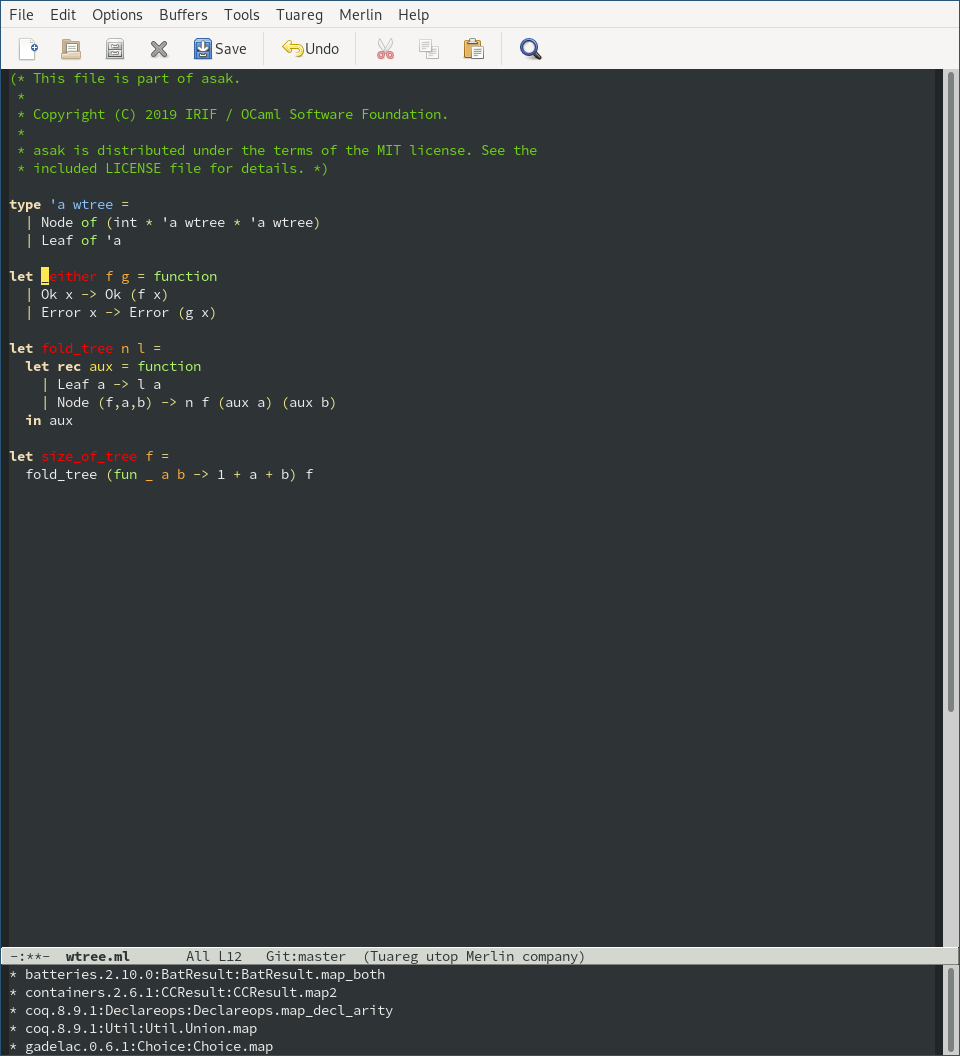
\includegraphics[scale=0.3]{anzad.png}
\end{figure}
\end{multicols}
\end{frame}

\begin{frame}
	\frametitle{Questions ?}
	\begin{center}
          \Large
		Merci de votre attention ! \\
                Merci à la Fondation OCaml !
	\end{center}
\end{frame}
\end{document}
